%%%%%%%%%%%%%%%%%%%%%%% file template.tex %%%%%%%%%%%%%%%%%%%%%%%%%
%
% This is a template file for Web of Conferences Journal
%
% Copy it to a new file with a new name and use it as the basis
% for your article
%
%%%%%%%%%%%%%%%%%%%%%%%%%% EDP Science %%%%%%%%%%%%%%%%%%%%%%%%%%%%
%
%%%\documentclass[option]{webofc}
%%% "twocolumn" for typesetting an article in two columns format (default one column)
%
\documentclass{webofc}
\usepackage[varg]{txfonts}   % Web of Conferences font
%
% Put here some packages required or/and some personnal commands
%
%
\begin{document}
%
\title{Event reconstruction in the BM@N experiment}
%
% subtitle is optional
%
%%%\subtitle{Do you have a subtitle?\\ If so, write it here}

\author{\firstname{P.~} \lastname{Batyuk}\inst{1}\fnsep\thanks{\email{pavel.batyuk@jinr.ru}} \and
  \firstname{D.~} \lastname{Baranov}\inst{1} \and
  \firstname{S.~} \lastname{Merts}\inst{1} \and
  \firstname{O.~} \lastname{Rogachevsky}\inst{1}
}

\institute{Veksler and Baldin Laboratory of High Energy Physics, JINR Dubna, 141980 Dubna, Russia}

\abstract{%
  In the article the main accent is put on development of software to be used within the BM@N experiment.
  The experiment is considered as a first step towards a fulfill realization of fixed target program at the NICA complex.
  A brief description of software used for reconstruction of track parameters in the inner tracker of the experiment is given.
  Some utmost urgent point like alignment procedure in automatic mode being made with the Millepede package fully integrated in the software is considered.
  Results illustrating a quality assurance of alignment performed with existing experimental data obtained from experimental runs and recent results,
  including methodological ones, got from a tracking procedure we are using for event reconstruction in the inner tracker are also presented.
  Importance of a precise geometry description, a realistic detector response via micro-simulations done for the GEM part of the inner tracker
  in order to be subsequently used when processing experimental data as well as our recent progress on this activity are discussed in the work.
}
%
\maketitle
%
\section{Experimental setup}
\label{setup}

BM@N (Baryonic matter at Nuclotron)~\cite{Baranov:2018cdk} is considered as a first step towards realization of physics program at the NICA complex.
It covers a fixed target program available at Nuclotron with extracted beams of different species.
The experiment had a set of technical runs mainly aimed to test sub-detector systems.
The last one took place on spring 2018 with argon and krypton beams available in a range of kinetic energies of 2.3 - 3.2 AGeV.

\begin{figure}[h]
  % Use the relevant command for your figure-insertion program
  % to insert the figure file.
  \centering
  \includegraphics[width=10cm,clip]{fig1.png}
  \caption{View of experimental setup in the last run.}
  \label{bmn}
\end{figure}

Schematic view of experimental setup is shown in fig.~\ref{bmn}. In the article main accent is put on development of algorithms of reconstruction
in relation to GEM (n.4 in fig.~\ref{bmn}) and silicon detectors (n.3 in fig.~\ref{bmn}). The GEM and silicon detectors form together inner tracker system of the experiment.
It consists of nine sensitive planes, in particular, three of them correspond to silicon detector and six to GEM.

\section{Reconstruction algorithm for inner tracker}
\label{hits}

Reconstruction of spatial coordinates of points produced by a charge particle on a sensitive element of detector serves as a necessary step towards finding tracks
and estimation of their parameters. These points are called ``hits''.

Algorithm to be used for reconstruction of hits consists of two subsequent stages: clusterization and search of hits by strip intersections.

Detectors for track reconstruction used in the inner tracker of the BM@N experiment have a microstrip readout. It leads to a presence of two-layer structure of strip assembly
in order to have a possibility to calculate spatial coordinates by making use intersections of fired strips.
Search for a cluster and its parameterization are done separately in each layer.
Generally speaking, a layer with a defined set of fired strips is considered as a one-dimensional discrete spectrum to be analyzed.
In course of this analysis one has to reveal cluster structures of peak form in the spectrum. Found clusters are parametrized thus giving us a set of parameters
which characterize each cluster. Among them the most important are position of center of gravity of the cluster along strip axis, width of the cluster and its total charge.
Positions of center found in two layers at the previous step describe average positions of fired strips to be intersected in order to get spatial coordinates of hit (see fig.~\ref{recoHits}).

\begin{figure}[h]
  % Use the relevant command for your figure-insertion program
  % to insert the figure file.
  \centering
  \includegraphics[width=5cm,clip]{fig2.png}
  \caption{Schematic interpretation of reconstruction algorithm.}
  \label{recoHits}
\end{figure}
The procedure described above is enhanced by additional post-processing algorithms aiming at noise filtering, unfolding of clusters located in close proximity etc.

Another important point to be stressed is a fact that use of detector planes based on strip readout has a big disadvantage revealing itself when obtaining a set of false
intersections called ``fakes'' (see fig.~\ref{fakes}).
\begin{figure}[h]
  % Use the relevant command for your figure-insertion program
  % to insert the figure file.
  \centering
  \includegraphics[width=8cm,clip]{fig3.png}
  \caption{Illustration of ``fake'' production.}
  \label{fakes}
\end{figure}
There are different ways to suppress them. It can be achieved on stage of detector construction as well as when doing a program post-processing of
existing data. Firstly, readout plane of detector is divided into small zones with its own set of strips. The smaller length of the strip the less number of intersections
obtained with other strips takes place. Secondly, to prevent production of ``fakes'', strips of two layers have a relatively small angle of intersection (stereo angle).
In particular, the GEM detectors we are using have the stereo angle of order of 15 degrees. At the same time, a value of stereo angle for silicon detectors of the inner tracker
is equal to 2.5 degrees. It should be stressed that decreasing the stereo angle too much leads to a big uncertainty when reconstructing Y-coordinate. A possible solution to reduce
the uncertainty follows pitch decrease (distance between strips), but it results to increasing number of channels of electronics and complication of detector. Presently, the pitch
values are 800 $\mu m$ for GEM and of order of 100 $\mu m $ for silicon detector.
A program post-processing aiming at preventing production of ``fakes'' takes place when doing signal filtering. It necessary to suppress noise as far as possible, to mark strips
that do not work correctly because of high contribution to ``fakes'' production. It is considered as a task of utmost importance with respect to experimental data processing.
Further, ``fake'' tracks obtained from ``fake'' hits are filtered by some criteria in course of tracking procedure.    

\subsection{Realistic simulations}
\label{simulations}
Data to be obtained from Monte Carlo simulations of passing of charged particles through geometry volumes via GEANT3/4 does not take into account specific aspect concerning
formation of signals in a detector setup. A simplified interpretation, e.g. Monte Carlo points describing exact positions of tracks without ``fake'' production and
other effects, is taken into account. It looks sufficient to get some basic characteristics of detector, but sounds inappropriately to describe and take into account a list of
realistic effects taking place when processing real experimental data.

In order to go towards realistic simulation of detector we developed a program model, applicable to the GEM detector, that uses information got from Garfield++
simulations~\cite{Pfeiffer:2018yam}.
These simulations use geometry characteristics of the GEM detector (distances between amplifying gaps), magnitude and orientation of electric and magnetic fields inside the gaps,
composition of gas mixture  as input. After the simulations performed, we have a possibility to produce clusters on readout plane with characteristics similar to those
we obtain with experimental setup.

The BM@N setup uses ``thick'' GEMs with a typical value of width close to 9 mm. Since they are located in inhomogeneous magnetic field, it is necessary to take into account its
influence. Due to the indicated width essential shifts of electrons by the Lorentz force take place. It leads to a biased position of cluster registered by readout plane.
For a gas mixture used in last experimental runs ($ArCO_{2}$(70:30)) at given magnitudes of electric field inside the amplifying gaps (1000:2500:3750:6300 V/cm) and magnetic field
(0.9 T) an average shift of cluster is of order of 1.7 mm.

All obtained parameters derived from simulations allowed us to calculate and take into account shifts as a function of magnetic field caused by the Lorentz force
when experimental data processing. Due to this, efficiency of reconstruction of real coordinates of hits has been essentially increased.

\section{Tracking}
\label{tracking}

An algorithm based on cellular automaton~\cite{CA} and integrated to the BmnRoot software~\cite{bmnroot} is used to reconstruct parameters of tracks of charged particles.
In this approach cell is defined and considered as a line segment connecting two hits pertaining to different planes of inner tracker.
The algorithm consists of the following steps:
\begin{enumerate}
\item Creation of cells.
  At this stage all possible connections between neighbouring detector planes are created. A restriction on maximal value of slope in ZX and ZY planes is used when creating cells. 
\item Calculation of cell states.
  The stage is done iteratively. % Number of iterations depends on number of planes of inner tracker.
  At first step all cells have a state equal to unity. Further, in course of iterations, if two cells have a common hit and similar slopes in ZX and ZY planes, then state of right
  cell is increased by unity. Iterations are done over all elements (planes) of inner tracker. It leads to calculation of final states for all cells.
\item Creation of candidates to be considered as future tracks.
  At this stage found cells are unified with their left neighbours if state difference is equal to unity. As a result, an array of candidates to be tracks consisting of a few cells,
  is created. A candidate is rejected if having less than four hits. ``Kept'' candidates are passed through procedures aimed to estimate vector of state and covariance matrix by a
  fit with circle.
\item Smooth of parameters of candidates.
  Candidates are processed by the Kalman filter to improve their parameters found at the previous step.
\item Sort of candidates.
  The stage is introduced in order to sort found candidates over number of hits and $\chi^{2}$-criterion to reject inappropriate candidates still kept via previous steps.
\item Selection of tracks.
  If two candidates sorted already have a shared hit, then preference is given to a candidate with less value of $\chi^{2}$ and larger number of hits. This candidate being considered from now
  as a track, is written to output array of found tracks.     
\end{enumerate}

The algorithm developed by our group can reconstruct curved tracks in magnetic field as well as straight ones in absence of magnetic field.
A set of quality assurance tests done with help of Monte Carlo input representing interactions of argon beam with kinetic energy of order of 3.2 AGeV with lead target showed reasonable values
of tracking efficiency, good precision of primary vertex and momentum reconstruction (see fig.~\ref{QA}).
Obtained average level of efficiency is closed to 80\% for a wide range of momentum. Also, a contribution of silicon part of inner tracker looks extremely important
when reconstructing primary vertex. It allows us to improve vertex resolution by factor of four.

\begin{figure}[h]
  % Use the relevant command for your figure-insertion program
  % to insert the figure file.
  \centering
  % \includegraphics[width=5cm,clip]{eff.png}
   \includegraphics[width=4.5cm,clip]{fig4b.pdf}
  \includegraphics[width=6.3cm,clip]{fig4a.pdf}
 % \includegraphics[width=5cm,clip]{momRes.png}
  \caption{Tracking efficiency and vertex resolution obtained in quality assurance tests.}
  \label{QA}       % Give a unique label
\end{figure}

The algorithm was used to reconstruct tracks in inner tracker obtained from existing experimental data recorded in the last experimental run.
In particular, it was used to perform track based alignment (Sect.~\ref{alignment}) of inner tracker.
As for recorded data with magnetic field, in fig.~\ref{spectra} are demonstrated momentum spectra for different targets as a function of different number of hits per track.
It is seen an increasing manifestation of spectators and light fragments for lighter targets that is in agreement with theoretical predictions.

\begin{figure}[h]
  % Use the relevant command for your figure-insertion program
  % to insert the figure file.
  \centering
  \includegraphics[width=5cm,clip]{fig5a.pdf}
  \includegraphics[width=5cm,clip]{fig5b.pdf}
  \caption{Momentum spectra of reconstructed charged particles for carbon (a) and lead (b) targets as a function of number of hits per track.}
  \label{spectra}       % Give a unique label
\end{figure}

A distribution of reconstructed primary vertex is shown in fig.~\ref{vertex}. Primary vertex is calculated by method of virtual planes.
At the moment, the obtained resolution is worse if compared with results from Monte Carlo (see fig.~\ref{QA}) thus challenging further improvements of the algorithm.   
\begin{figure}[h]
  % Use the relevant command for your figure-insertion program
  % to insert the figure file.
  \centering
  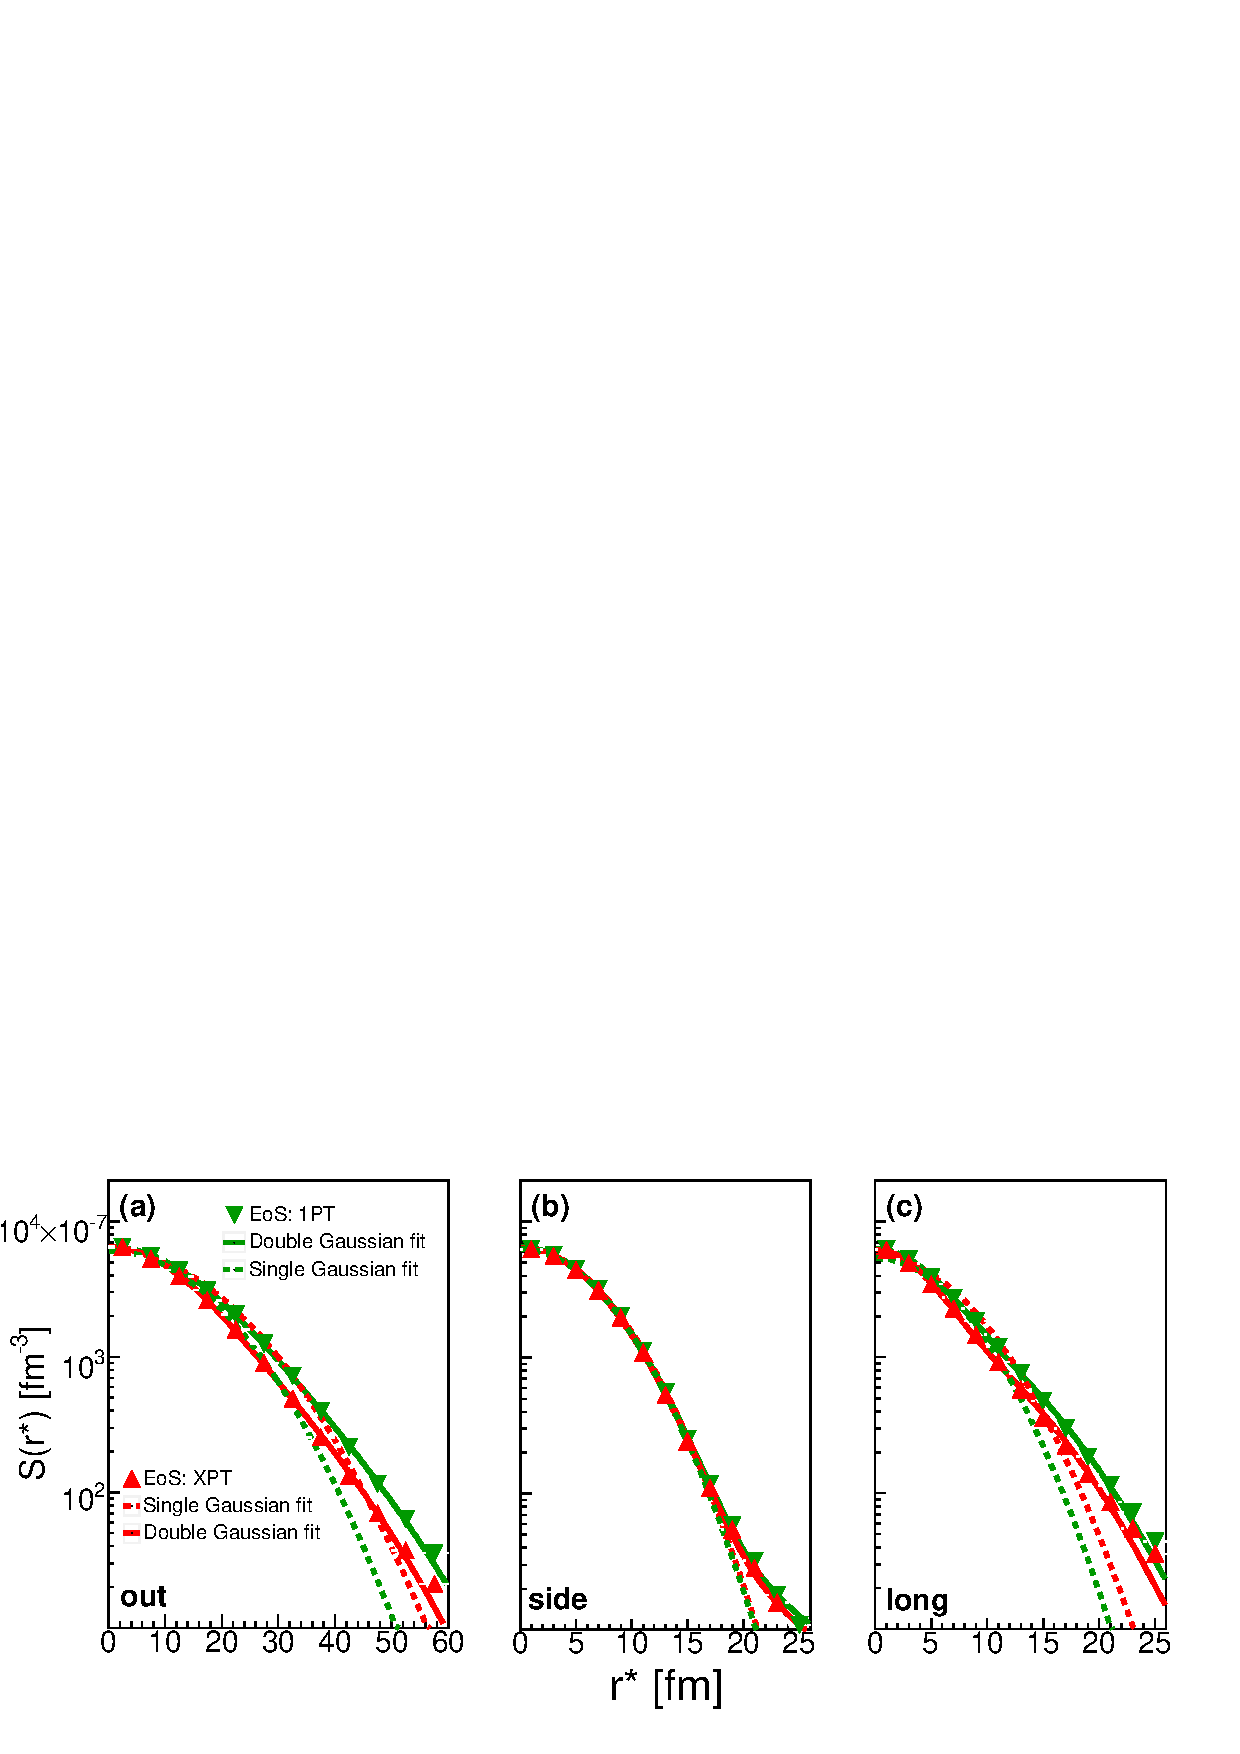
\includegraphics[width=5cm,clip]{fig6.pdf}
  \caption{Distribution of z-coordinate of primary vertex. Interactions with lead target are used for analysis.}
  \label{vertex}       % Give a unique label
\end{figure}


\section{Alignment}
\label{alignment}

Track based alignment is considered as a task of utmost importance.
The BmnRoot framework has a well developed software ALCOPACK (ALignment COrrection PACKage) to be used for alignment of inner tracker.

The software is based on the Millepede-II formalism~\cite{Blobel:2002ax}.
At present, a track model used does not take into account material effects and allows one a simple parameterization by straight line.
Use of more sophisticated track models taking into account a wider set of realistic effects is being tested now.
Moreover, the software allows to include or exclude detectors from alignment thus giving a possibility to align them separately.
A mechanism of constraints based on the Lagrange multipliers can be used to prevent a total shift of detector.

In fig.~\ref{align} are shown distributions of z-coordinate of primary vertex before and after alignment done.
\begin{figure}[h]
  % Use the relevant command for your figure-insertion program
  % to insert the figure file.
  \centering
  \includegraphics[width=5cm,clip]{fig7a.pdf}
  \includegraphics[width=5cm,clip]{fig7b.pdf}
  \caption{Distribution of z-coordinate of primary vertex before (a) and after (b) alignment. Used data are recorded without magnetic field.}
  \label{align}       % Give a unique label
\end{figure}
As a result, width of the distribution has been reduced by factor of two. Positions of some trigger detectors (BC3 and Si trigger) are
distinguished better after the alignment done.  

\section*{Acknowledgments}
We thank N. Kutovskiy and his team~\cite{jinrCloud} for a given possibility to use well equipped JINR cloud infrastructure for the calculations we were doing when processing experimental data.
We are grateful to M.~Kapishin, N.~Zamiatin, E.~Zubarev for fruitful discussions and considerations when the work was initiated. 


\begin{thebibliography}{}
\bibitem{Baranov:2018cdk} 
  D.~Baranov, M.~Kapishin, T.~Mamontova, G.~Pokatashkin, I.~Rufanov, V.~Vasendina and A.~Zinchenko,
  %``The BM@N Experiment at JINR: Status and Physics Program,''
  KnE Energ.\ Phys.\  {\bf 3}, 291 (2018).
  DOI:10.18502/ken.v3i1.1757
  %%CITATION = doi:10.18502/ken.v3i1.1757;%%
 

\bibitem{Pfeiffer:2018yam}
  D.~Pfeiffer {\it et al.},
  %``A Geant4/Garfield++ and Geant4/Degrad Interface for the Simulation of Gaseous Detectors,''
  arXiv:1806.05880 [physics.ins-det].
  %%CITATION = ARXIV:1806.05880;%%
  
\bibitem[Glattauer et al.(2012)]{CA} Glattauer, R., Fr{\"u}hwirth, R., Lettenbichler, J., and Mitaroff, W.\ 2012, arXiv:1202.2761
\bibitem{bmnroot} Gertsenberger, K., Merts, S., Rogachevsky, O. et al. Eur. Phys. J. A (2016) 52: 214. https://doi.org/10.1140/epja/i2016-16214-y
  
\bibitem{Blobel:2002ax}
  V.~Blobel and C.~Kleinwort,
  %``A New method for the high precision alignment of track detectors,''
  hep-ex/0208021.
  %%CITATION = HEP-EX/0208021;%%
  %82 citations counted in INSPIRE as of 13 Nov 2018

\bibitem{jinrCloud} A.V. Baranov,  N.A. Balashov, N.A. Kutovskiy, R.N. Semenov, JINR cloud infrastructure evolution // Physics of Particles and Nuclei Letters,
  ISSN 1547-4771, eISSN: 1531-8567, 2016, vol. 13, No. 5, pp. 672–675. DOI: 10.1134/S1547477116050071
\end{thebibliography}


\end{document}

% end of file template.tex
